\chapter{Architectural Overview}


ACE is split into three independent layers. Each layer has a well-defined 
interface between the adjoining layers and well-defined responsibilities. 
A layer implementation can be replaced easily.

\begin{figure}[H]
 \centering
 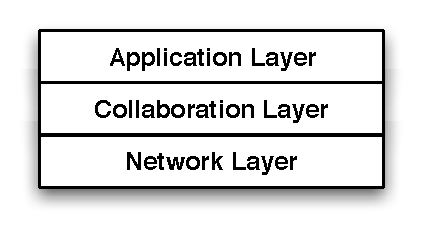
\includegraphics[width=6.6cm,height=3.42cm]{../images/layers.eps}
 \caption{The Layers of ACE}
\end{figure}

\paragraph{Application Layer:} The application layer consists mainly in the 
graphical user interface. The layer implementation in ACE is built with
Java Swing.

\paragraph{Collaboration Layer:} The collaboration layer provides the
collaborative editing functionality to the application layer. It hosts the core
consistency control algorithm, which is based on the concept of operational 
transformation. By replacing the collaboration layer it would be theoretically 
possible to replace the employed consistency control algorithm. Further it uses 
the network layer for all network related functionality.

\paragraph{Network Layer:} The network layer is the lowest layer of ACE. It 
provides networking functionality to the collaboration layer. The two most 
important features are discovery of users and documents as well as communication 
with other users and sessions. Replacing the network layer allows to use a 
different network technology and/or a different protocol.



\section{Interface Application/Collaboration Layer}
The main class in the collaboration layer is the \texttt{CollaborationService}.
It is the entry point for an application layer. The main functionality 
exposed by the collaboration service are:
\begin{itemize}
 \item discovery of users and documents
 \item publishing of local documents
 \item registering invitation callback
\end{itemize}


\subsection{Collaboration Service}

\begin{figure}[H]
 \centering
 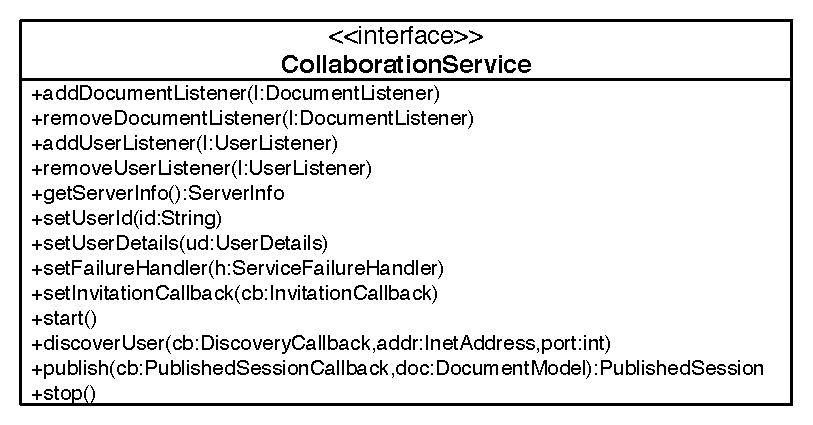
\includegraphics[width=13.83cm,height=7.27cm]{../images/finalreport/architecture_collaborationservice_uml.eps}
 \caption{CollaborationService Interface}
\end{figure}

The \texttt{CollaborationService} has to be initialized before it can
be used. This includes typically the following:

\begin{itemize}
 \item setting local user id
 \item setting local user details
 \item adding listeners
 \item setting callbacks
\end{itemize}

Each running instance of ACE needs a unique user id. This id is used to uniquely
identify users. The user id is set with the \texttt{setUserId} method. The
user details (at the moment just the nickname of the user) are set with
\texttt{setUserDetails}.

Further, the \texttt{CollaborationService} provides the possibility to set a
\texttt{ServiceFailureHandler} 
(see figure \ref{fig:archoverview.servicefailurehandler}). 
This failure handler is notified about 
service failures and is set with the \texttt{setFailureHandler} method. 
A typical service failure occurs if the port used by
ACE is already in use by another application. The failures passed to that
handler are really intended to be on the service level. Session level failures
are handled differently (see \ref{sect:archoverview.sessionfailure}). 

\begin{figure}[H]
 \centering
 
\includegraphics[width=8.71cm,height=2.15cm]{../images/finalreport/architecture_servicefailurehandler_uml.eps}
 \caption{ServiceFailureHandler Interface}
 \label{fig:archoverview.servicefailurehandler}
\end{figure}


The registration of listeners as well as the setting of the invitation 
callback are discussed in the following.

Once all the necessary setup steps have been performed, the
\texttt{CollaborationService} can be started with a call to the
\texttt{start} method. At the end of the lifecycle of the
service, the \texttt{stop} method should be called.

The \texttt{getServerInfo} method can be used to get the local 
\texttt{ServerInfo} object, which specifies the IP and port of the
local server. Note that this information may not be available right
from the beginning, as it could be dynamically be determined when the
service is started. The application should therefore poll for that information
until it is available (e.g. with a timer).


\subsection{Discovery}
The collaboration service provides a listener registration mechanism for
users and documents. The corresponding methods are \texttt{addUserListener}
and \texttt{addDocumentListener}. These listeners are notified whenever a
new user or document is discovered by the underlying network layer. The two 
listener interfaces are pretty similar. 

\begin{figure}[H]
 \centering
 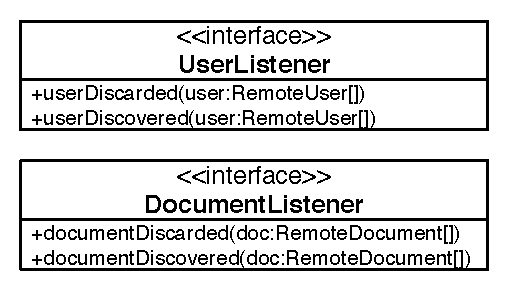
\includegraphics[width=8.47cm,height=4.97cm]{../images/finalreport/architecture_listener_uml.eps}
 \caption{DocumentListener and UserListener Interfaces}
\end{figure}

The passed in objects are instances of \texttt{RemoteUser} and
\texttt{RemoteDocument} respectively. The user objects have a \texttt{name}
property and documents have a \texttt{title} property. Further, they support
property change events that are used to notify registered 
\texttt{PropertyChangeListener} instances about property value changes. 
The collaboration layer guarantees that for each unique user and document
there is only one \texttt{RemoteUser} and \texttt{RemoteDocument}. This makes
it possible to register \texttt{PropertyChangeListener}s to be notified about
changes to the user name and document title. 

\begin{figure}[H]
 \centering
 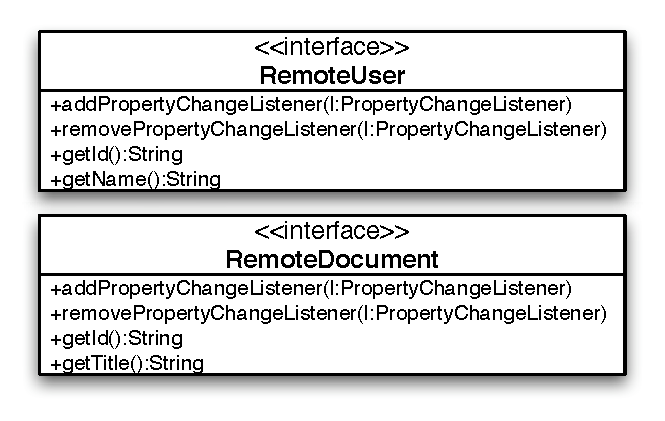
\includegraphics[width=10.69cm,height=6.56cm]{../images/finalreport/architecture_userdocument_uml.eps}
 \caption{RemoteUser and RemoteDocument Interface}
\end{figure}


The
\texttt{RemoteDocument} objects have also a property that returns the
\texttt{RemoteUser} for the publisher of the document.


\subsection{Explicit User Discovery}
The described discovery mechanism relies on the services of the network layer.
It usually relies on IP multicast, which is most likely not available outside
of the local subnet. ACE provides therefore an explicit way to discover users.
The \texttt{CollaborationService} has a method \texttt{discoverUser} with
three parameters. A \texttt{DiscoveryCallback} is used to report the result
of the discovery, a \texttt{InetAddress} specifying the host, and a port.

\begin{figure}[H]
 \centering
 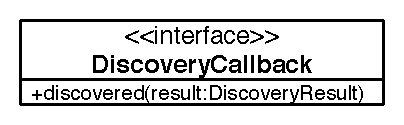
\includegraphics[width=8.47cm,height=2.19cm]{../images/finalreport/architecture_discoverycallback_uml.eps}
 \caption{DiscoveryCallback Interface}
\end{figure}

The callback is notified about the result of the discovery. The passed in
\texttt{DiscoveryResult} has a status and a status message. If the status
is equal to \texttt{DiscoveryResult.SUCCESS} the discovery succeeded. The
discovered user is returned through the normal code path, i.e. the
registered \texttt{UserListener} objects receive a notification.

\begin{figure}[H]
 \centering
 
\includegraphics[width=5.57cm,height=2.54cm]{../images/finalreport/architecture_discoveryresult_uml.eps}
 \caption{DiscoveryResult}
\end{figure}


\subsection{Joining Documents}
\label{sect:archoverview.join}
\texttt{RemoteDocument} instances have a method \texttt{join}. This join
method can be used to join a remote document. All that is needed to
join a document is to register a \texttt{DocumentListener} with the 
\texttt{CollaborationListener} and call join on a discovered document.

The \texttt{join} method is designed to return immediately. Join is a 
potentially long running operation. First, the join request has to be sent
to the publisher. Second, it might take some time to transfer the document
content over the network. And last but not least, joining might need the 
approval of the publisher, which might take even longer. Thus, it is a sensible 
design decision to make this method non-blocking.

The result of join request is communicated to an object passed to the
\texttt{join} method implementing the \texttt{JoinCallback} interface.

\begin{figure}[H]
 \centering
 
\includegraphics[width=9.07cm,height=2.58cm]{../images/finalreport/architecture_joincallback_uml.eps}
 \caption{JoinCallback Interface}
\end{figure}

Depending on the outcome of the join request, either \texttt{accepted} or
\texttt{rejected} is called. The \texttt{accepted} method takes an argument
of type \texttt{Session} and returns a \texttt{ParticipantSessionCallback}. 
The session
is the object that represents a collaborative editing session. It is
implemented by the collaboration layer and passed to the application layer.
The \texttt{ParticipantSessionCallback} in turn is returned by the application 
layer to the collaboration layer and is used by it to return received operations
and caret updates from other participants in the session.


\subsection{Publishing Documents}
To publish a document, the \texttt{CollaborationService} method \texttt{publish}
is used. The method has two parameters. The first is the session callback
for a published session (\texttt{PublishedSessionCallback}). The second method 
is the \texttt{DocumentModel}
of the document to be published. The \texttt{DocumentModel} contains the
document content, the title, as well as the current caret position of the
publisher. The collaboration service in turn returns an object of type
\texttt{PublishedSession}, which is used both to control the session as well
as sending operations and updates to the caret position.


\subsection{Inviting Users}
\label{sect:archoverview.invitingusers}
The \texttt{PublishedSession} has a method \texttt{invite} to invite users.
The invite method has as single parameter of type \texttt{RemoteUser}. 
The invite method is non-blocking, i.e. it
returns immediately. If the user accepts the invitation, he is added to the
list of participants of the session. The API does not provide a way to return
a feedback to the application layer whether the invitation is accepted.
Future versions may improve in that area and add a callback interface for
the invitation result.


\subsection{Receiving Invitations}
The \texttt{CollaborationService} has a method to register an
\texttt{InvitationCallback}. This callback is notified whenever another user
tries to invite the local user. 

\begin{figure}[H]
 \centering
 
\includegraphics[width=7.48cm,height=2.15cm]{../images/finalreport/architecture_invitationcallback_uml.eps}
 \caption{InvitationCallback Interface}
\end{figure}

The passed in \texttt{Invitation} allows to retrieve the document for which
the user is invited as well as the publisher of the document. The
methods are \texttt{accept} and \texttt{reject}. They represent
the user actions of accepting or rejecting an invitation. 

\begin{figure}[H]
 \centering
 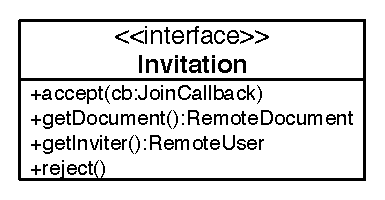
\includegraphics[width=6.60cm,height=3.76cm]{../images/finalreport/architecture_invitation_uml.eps}
 \caption{Invitation Interface}
\end{figure}

The \texttt{accept} method has as parameter a \texttt{JoinCallback}. This
callback is used exactly in the same way as the \texttt{JoinCallback} passed
to the \texttt{join} method of the \texttt{RemoteDocument} 
(see \ref{sect:archoverview.join}).


\subsection{Communicating with a Session}
Until now, we have not discussed how to communicate with a session. An
editing session is represented by the \texttt{Session} interface.
We have shown several ways to get a \texttt{Session} object:

\begin{itemize}
 \item joining a discovered remote document
 \item accepting an invitation
 \item publishing a local document (\texttt{PublishedSession})
\end{itemize}

All those ways have one thing in common: the application layer has to pass a 
\texttt{SessionCallback}
(in case of publish a \texttt{PublishedSessionCallback} and in every
other case a \texttt{ParticipantSessionCallback}) to the collaboration
layer. There are always these two objects, a \texttt{Session} and
a \texttt{SessionCallback}. The \texttt{Session} is used by the application
layer to send events to collaboration layer and a \texttt{SessionCallback}
is used to notify the application layer about session related events from the 
collaboration layer. Figure \ref{fig:archoverview.sessionandcallback} depicts 
this situation.

\begin{figure}[H]
 \centering
 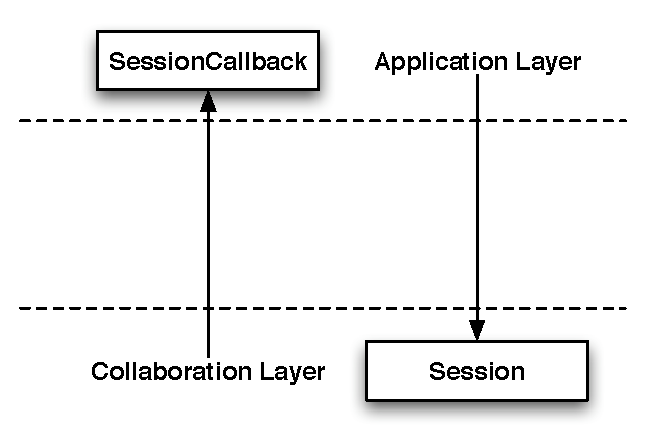
\includegraphics[width=10.37cm,height=7.02cm]{../images/finalreport/architecture_session_sessioncallback.eps}
 \caption{Session and SessionCallback}
 \label{fig:archoverview.sessionandcallback}
\end{figure}

The figure \ref{fig:archoverview.session} shows the \texttt{Session} interface
hierarchy.

\begin{figure}[H]
 \centering
 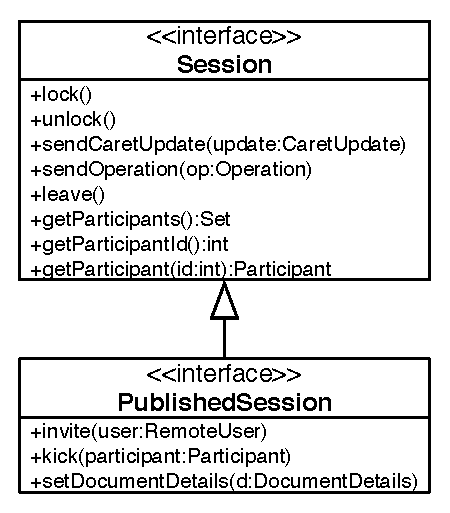
\includegraphics[width=7.69cm,height=8.75cm]{../images/finalreport/architecture_session_uml.eps}
 \caption{Session and PublishedSession Interface}
 \label{fig:archoverview.session}
\end{figure}


\subsubsection{Locking}
In order that the system can guarantee the consistency of the replicas, we
must employ a locking scheme in the session and the document model of
the application layer implementation. While transforming messages, nobody
can be allowed to modify the document. 

Before determining the index and the text of a local operation, the session must
be locked. This ensures that from the point where the operation is determined
to the point where a request is created for the operation no other text is
inserted. Failing to do that would potentially result in an invalid index for
the local operation, as a processed remote operation could shift the text.

On the other hand for the same reasons, the session should also ensure with a 
lock that the local document model does not change while a remote request is 
processed.

The \texttt{SessionCallback} has a method \texttt{getLock}, from which
the collaboration layer gets a lock from the application layer. This
lock is used inside the session as well as it is available through the
\texttt{lock} and \texttt{unlock} methods. Make sure that for each call to
\texttt{lock} there is a matching \texttt{unlock} call. To be sure that unlock
is called, it must be placed inside a finally block.

\begin{figure}[H]
 \centering
 \small{\begin{verbatim}
 Session session = ...;
 session.lock();
 try {
   Operation op = ...;
   session.sendOperation(op);
 } finally {
   session.unlock();
 }
 \end{verbatim}}
 \caption{Proper locking of a Session}
\end{figure}

The documentation of the application layer (see \ref{chap:applicationlayer}) 
shows how the lock is implemented in our application layer implementation.


\subsubsection{Sending Operations}
The \texttt{sendOperation} and \texttt{sendCaretUpdate} methods are used to send 
locally generated operations or
caret updates to the other participants in the session. The \texttt{leave}
method allows to leave the session, i.e. stop participating. The participant
related methods allow to access the currently participating users. These
methods return objects implementing the \texttt{Participant} interface. This
interface has
two methods, one to get the \texttt{RemoteUser} and one to get the participant
id.

\begin{figure}[H]
 \centering
 
\includegraphics[width=4.97cm,height=2.1cm]{../images/finalreport/architecture_participant_uml.eps}
 \caption{Participant Interface}
\end{figure}

A participant id is a session-wide unique identifier for a user. They are given
to a user when he joins a session by the publisher of the session. The local
participant id can be retrieved by the \texttt{getParticipantId} method.

The interface used by the collaboration layer to notify the client of the
session about events is the \texttt{SessionCallback} interface.


\subsubsection{PublishedSession}
The \texttt{PublishedSession} has some additional methods that correspond
to the additional actions available to the publisher of a document. The
publisher can change the name of the document through the
\texttt{setDocumentDetails} method. This happens most likely because the
publisher saves the document under a different name.
The \texttt{invite} method we have already seen in action in the section
\ref{sect:archoverview.invitingusers}.

Last but not least, the \texttt{kick} method can be used to kick a
participant from the session. This gives the publisher the possibility to
ban a user from the session.


\subsection{Session Callbacks}
\begin{figure}[H]
 \centering
 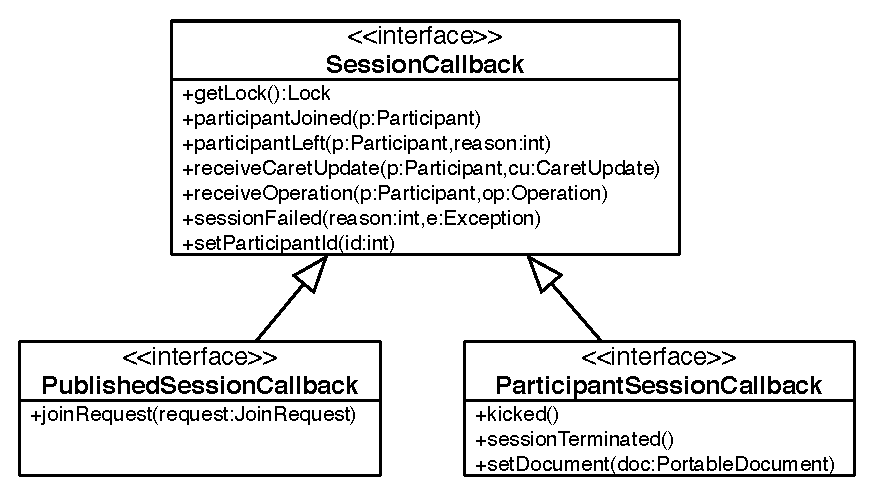
\includegraphics[width=14.89cm,height=8.47cm]{../images/finalreport/architecture_sessioncallback_uml.eps}
 \caption{SessionCallback Interfaces}
 \label{fig:archoverview.sessioncallback}
\end{figure}

The \texttt{SessionCallback} contains the methods common to both session types:
the participant and the publisher session. The 
\texttt{ParticipantSessionCallback} adds method that can only be called for
participants.


\subsubsection{Initialization and Termination of Participant Sessions}
When joining a document or accepting an invitation the session is passed to
the \texttt{JoinCallback} \texttt{accepted} method. This method has a
parameter of type \texttt{ParticipantSessionCallback}. The first two
methods called on that callback object are \texttt{setParticipantId}, which 
communicates the assigned participant id of the local participant, and 
\texttt{setDocument}, which sets the document. After these methods are called
all the other methods can be called by the session.

The \texttt{setDocument} method gets a \texttt{PortableDocument} instance
as parameter. It represents the document content at join time. A portable
document consists of a set of participants, their selections, as well as
a collection of fragments. A fragment is simply a continous run of text
belonging to one particular participant.

\begin{figure}[H]
 \centering
 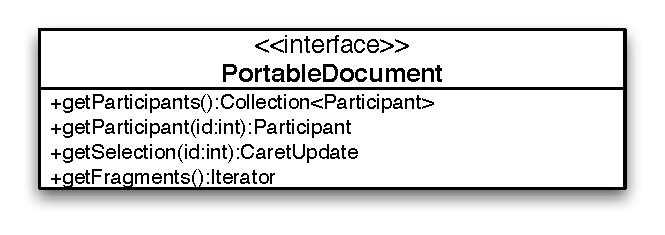
\includegraphics[width=10.69cm,height=3.42cm]{../images/finalreport/architecture_portabledocument_uml.eps}
 \caption{PortableDocument Interfaces}
\end{figure}

The \texttt{kicked} method is called when the local participant
has been kicked from the session. A participant is typically kicked from
the session when he does not behave well. The \texttt{sessionTerminated}
method is called when the publisher conceals the published document. 

Additionally a session can fail. Session failures are common to publisher
sessions too and are described in the next section.


\subsubsection{Session Failures}
\label{sect:archoverview.sessionfailure}
The \texttt{sessionFailed}
method is used by the collaboration layer to notify the application layer
about a failed session. Reasons for this include failing network connection
to the publisher or unrecoverable situations in the collaboration or network
layer. The session should no longer be used after a call to 
this method.


\subsubsection{Reception}
The callback has methods to notify the client of the session about caret
updates and operations from other participants in the session. These methods
are named \texttt{receiveOperation} and \texttt{receiveCaretUpdate}
and accept both a \texttt{Participant} object
as well as either an \texttt{Operation} or a \texttt{CaretUpdate}.


\subsubsection{Participation Events}
The \texttt{participantJoined} and \texttt{participantLeft} methods are used to
notify the callback about
participants that joined or left the session. The initial set of participants
can be retrieved from the session when the document is set with
the \texttt{getParticipants} method.


\subsubsection{PublishedSessionCallback}
The \texttt{PublishedSessionCallback} method has a single additional method
\texttt{joinRequest} which has a parameter of type \texttt{JoinRequest}. It
is invoked whenever a user tries to join the session. The publisher of the
session can then decide if the user is allowed to join. The \texttt{JoinRequest}
has a single property of type \texttt{RemoteUser}, which is the user that 
tries to join. The request can either be accepted or rejected with the 
corresponding methods \texttt{accept} or \texttt{reject}.

\begin{figure}[H]
 \centering
 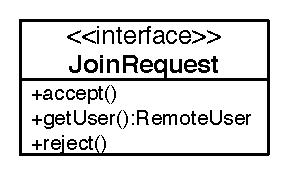
\includegraphics[width=4.97cm,height=3.03cm]{../images/finalreport/architecture_joinrequest_uml.eps}
 \caption{JoinRequest Interfaces}
\end{figure}



\section{Interface between Collaboration and Network Layer}
In the last section we had a look at the interface between the application and
the collaboration layer. The collaboration layer itself cannot implement a
collaborative editor on itself. It needs a layer that provides the networking
functionality. The networking layer provides exactly that functionality to
the collaboration layer. It is not used directly by the application layer.

\subsection{Network Service}
The \texttt{NetworkService} interface is the entry point into the network layer.

%\begin{figure}[H]
% \centering
% \includegraphics[width=11.11cm,height=7.62cm]{../images/design/network-uml-%service.eps}
% \caption{UML of NetworkService}
% \label{fig:networkservice interface}
%\end{figure}

\subsection{Network Service Callbacks}

